\item Siehe Skizze \ref{ex-trigonometry-1-img-b}. Wir erhalten die beiden Gleichungen:

\begin{alignat*}{3}
(i)  \;  & L \cdot \cos(\alpha)  &&= L - h \\
(ii) \; &  L \cdot \sin(\alpha)  &&= w
\end{alignat*}

($w=21cm$, $h=10cm$, $\alpha$: Winkel zwischen der Senkrechten und der geneigten Lilie, $L$: gesuchte Tiefe des Sees)

Zur Lösung bilden wir die Summe der Quadrate beider Gleichungen:

$$(i)^2+(ii)^2 = L^2 (\cos^2(\alpha) + \sin^2(\alpha)) = (L-h)^2 + w^2$$

Da nun $\cos^2(\alpha) + \sin^2(\alpha) = 1$ gilt (Satz des Pythagoras)

$$ L^2 = L^2 + h^2 - 2Lh + w^2$$
$$\implies 0 = h^2-2Lh+w^2$$
$$\implies L = \frac{h^2+w^2}{2h}$$

Wir setzen die gegebenen Werte ein und erhalten für die Tiefe des Sees:

$$L=\frac{10^2\cdot\text{inch}^2 + 21^2\cdot\text{inch}^2}{2\cdot 10 \cdot\text{inch}} \approx 27,0 \text{ inch} = 69 \text{ cm}$$

Der Neigungswinkel beträgt dann $\alpha = \arcsin(\frac{w}{L})= \arcsin(\frac{21}{69}) \approx 17,7 ^ \circ$.

\begin{figure}[ht]
	\centering
	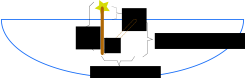
\includegraphics[width=0.75\textwidth]{../tex-snippets/ex-trigonometry-1-img-b.png}
	\caption{Skizze zur Rätselaufgabe.}
	\label{ex-trigonometry-1-img-b}
\end{figure}

